\documentclass[12pt, letterpaper]{article}
\usepackage{helvet} % Use Helvetica (or any other sans-serif font)
\usepackage{setspace} % Package for adjusting line spacing
\usepackage{graphicx} % Package for including graphics
\usepackage{dcolumn}
\usepackage{placeins}
\usepackage{natbib}
\usepackage{subcaption}
\usepackage{float}
\bibliographystyle{econ}
\usepackage[letterpaper, margin=1in]{geometry}%1.25

\begin{document}
\title{Measuring Knowledge Capital Risk} % Title in sans-serif font
\author{Pedro H. Braz Vallocci \\ University of California, Santa Cruz} % Author name and affiliation in sans-serif font

\newcommand{\ffo}{dicfullmc10thr10defnob5noa0_8_4t}

\newcommand{\insertfigure}[2]{
\begin{figure}[h!]
  \centering
  \includegraphics[width=0.8\textwidth]{\ffo/#1}
  \caption{#2}
  \label{fig:#1}
\end{figure}
}


\maketitle % Print the title, author, and date

\onehalfspacing % Set double spacing

\section{Introduction}

The transition towards a service- and knowledge-based economy has been accompanied by a sharp increase in intangible assets, most notably in research and development (R\&D). Knowledge capital, defined as a firm's accumulated investments in R\&D, accounts for an increasing share of public firms' valuation and has a different risk profile than physical capital. For example, knowledge capital-heavy firms are more exposed to the loss of key talent and changes in patent enforcement. However, to the best of my knowledge, there are no references in the literature that seek to understand if there are differences in risk premia among firms with different levels of knowledge capital and if agents are pricing in a sudden risk of economic disaster in knowledge capital. My paper seeks to fill this gap.

Spending on intangible assets qualifies as an investment since it reduces current consumption to increase future consumption \citep{Corrado2009-kd, Corrado2009-hk}. Moreover, endogenous growth models, such as models with expanding varieties \citep{Romer1990-tw}, and with quality ladders \citep{Grossman1991-pz, Atkeson2019-wz}, imply that research expenses can spur growth.

The two latter models consider R\&D as intermediate expenses. However, supply-side valuation models such as \citep{Belo2013-ys} argue that not only quasi-fixed physical capital and labor inputs but also knowledge and brand capital can determine a firm's market value. \emph{Knowledge capital} is defined as a firm's accumulated investments in R\&D. \emph{Brand capital} is defined as a firm's accumulated expenses in advertising \citep{Belo2019-iz}; \emph{organization capital} is defined as the set of unique systems and processes employed in an enterprise, which increases with a firm's managerial quality scores \citep{Eisfeldt2013-ad, Bloom2007-gl}. Knowledge capital, brand capital, and organization capital are components of a firm's intangible capital.

\cite{Hall2001-ni, McGrattan2001-kc, Vitorino2014-yd, Eisfeldt2020-ec, Li2014-zp} confirm that intangible capital matters for aggregate stock market valuations and, more specifically, firm-level valuations. \citep{Corrado2009-kd} estimated total intangible capital in 2003 to be 3.6 trillion, half of which as scientific and non-scientific R\&D capital. \citep{Crouzet2021-ic} found that the omission of knowledge capital and its associated rents can explain up to 2/3 of the investment gap (the difference between marginal $q$ and average $Q$) in R\&D intense sectors such as Healthcare and Chemicals.

However, equating the omission of intangible and knowledge capital to a mere mismeasurement of a firm's book value is misleading since intangible capital has unique characteristics and thus cannot be lumped together with physical capital. \citep{Autor2020-rw, Unger2019-ip} shed light on a "scale-biased technological change" in R\&D-heavy firms. Greater output scalability, the absence of geographical constraints for input sourcing or output distribution, and the greater importance of network effects lead to a "winner-takes-most" outcome in some industries (i.e., an uneven market power distribution) and a declining labor share, consistent with \citep{Barkai2020-gi}.

Moreover, R\&D-driven technological innovation, while generating research externalities in the form of knowledge available to the rest of society, may also be a force for creative destruction \citep{Schumpeter1939-er} if it leads to mere resource reallocation across firms. Therefore, it is not evident that private-led innovation increases aggregate output. \citep{Kogan2017-fx, Garcia-Macia2019-mg} show that innovation has a net effect of accelerating aggregate output and that own-product improvements by incumbents are more important than creative destruction.

R\&D-intensive firms are also more likely to offshore profit shifting, i.e., to license their intellectual property rights to offshore subsidiaries in order to accrue derived profits at tax-havens. Compared to non-R\&D-intensive firms (e.g., construction), it is easier to decouple the physical location of intellectual property production from its point of sale. Offshore profit shifting has grown since the 2000s, which coincides with the beginning of the productivity growth slowdown \citep{Fernald2015-io}. Adjusting for offshore profit shifting adds 2.1 log percentage points to R\&D-heavy firms, which is ten times larger than for non-R\&D. Labor productivity in R\&D-intensive firms has also grown much faster than in non-R\&D firms \citep{Guvenen2021-yh}.

The riskiness of intangible assets differs systematically from tangible ones \citep{Hansen2005-xe}. \citep{Eisfeldt2013-ad} points out that shareholders cannot entirely appropriate the cash flows from the key talent of the firm since the firm must always compensate key talent by its outside option. \citep{Eisfeldt2018-iy} shows that key talent partially owns the cash flow from intangible capital in the form of equity, finding that almost 40\% of compensation to high-skilled labor happens as equity-based pay. Finally, \citep{Ai2019-wd} predicts that collateralizable assets, which do not include some categories of intangibles, provide insurance against aggregate shocks in the economy and should earn a lower expected return.

Specifically, knowledge capital is risky. Firms spend on R\&D to increase their future profitability, which is not guaranteed. For example, research conducted by a pharmaceutical firm can lead to successful new drugs that lead to patent rents for several years or to no result at all. The riskiness of innovation firms, and the growing empirical dispersion of Tobin's q, also explains the relation between Tobin's q and aggregate investment has become tighter since the mid-1990s \citep{Andrei2019-bh}. The riskiness of a financially constrained firm increases with its R\&D intensity \citep{Li2011-ay}. Besides the uncertainty of research investments, a firm is also susceptible to writing off part of its knowledge capital, e.g., when it narrowly loses a patent race \citep{Peters2017-fl}.

Knowledge capital heavy firms are especially susceptible to loss of key talent. \citep{Eisfeldt2013-ad} find that firms are more likely to list "loss of key talent" as a risk factor in their 10-K reports when they have high organization capital. It makes sense that the same pattern is valid for knowledge capital heavy firms, which are highly dependent on specialized and scarce workforce.

Firms vulnerable to loss of key talent are especially susceptible to immigration-related risks, e.g., the H-1B visa annual quota shortages. The H-1B visa, introduced with the Immigration and Nationality Act of 1990, established temporary renewable visas for college-educated specialty professional workers, most of whom work in STEM occupations. \citep{Peri2015-qt} shows that the growth in foreign-STEM workers may explain between 10 and 25\% of the aggregate productivity growth and 10\% of skill-bias growth between 1990 and 2010.

Following previous literature on time-varying disaster risks, such as \citep{Gabaix2012-kw, Barro2006-pt, Rietz1988-ds}, \citep{Gourio2012-nt} shows that increases in the risk of an economic disaster can lead to an increase in risk premia and a decrease in unemployment and output. My work will develop upon \citep{Gourio2012-nt} to consider a knowledge capital heavy economy, and investigate if agents are pricing in the risk of sudden drops in the efficiency of knowledge investment (e.g., due to shortage of skilled workforce) or sudden firm-specific write-offs ("disasters") of knowledge capital (e.g., due to weakening in patent laws).

The current methods of identifying knowledge-heavy firms have proven to be insufficient due to a number of key issues. Firstly, there is a lack of consistency in the standards for R\&D reporting across industries and firms. This discrepancy is further compounded by the fact that some firms do not disclose their R\&D expenditure in their annual reports, making it challenging to accurately determine their level of knowledge intensity.

Secondly, the measures used to identify intangible assets, typically through indirect measures like Selling, General and Administrative expenses (SG\&A), include components that are not related to knowledge, such as organizational capital. This can blur the distinction between knowledge-heavy and non-knowledge-heavy firms.

Lastly, relying on patents as a measure of a firm's knowledge intensity only tells part of the story. While patents reflect the final outcomes of R\&D investments, they do not account for the internal learning processes that take place within firms, thus potentially undervaluing those that invest heavily in internal knowledge development, even if they do not have a high patent output.

Considering these shortcomings, several research questions emerge: Firstly, is it possible to better identify knowledge-heavy firms by performing text analysis on the risk factors reported in their annual reports? By analyzing the language and terminology used, can we glean more information about the firm's knowledge intensity?

Secondly, if we can indeed identify knowledge-heavy firms in this manner, does this information influence how agents price these firms? In other words, do market participants factor in different risks for knowledge-heavy firms compared to non-knowledge-heavy firms?

Finally, we must question if using topic modeling to categorize the firms' self-declared risk factors can provide a more sensible and accurate categorization of firms by risk. By examining the topics that firms themselves identify as risks, can we create a more nuanced classification system for firms based on the nature and magnitude of their risk exposure?

\section{Methodology and Data}

\subsection{Latent Dirichlet Allocation (LDA)}

In this study, I use Latent Dirichlet Allocation (LDA), a topic modeling technique, to identify latent topics within a comprehensive corpus of 121,839 firm annual reports spanning the years 2006 to 2022. This approach allows me to uncover patterns and themes in the data that may not be immediately apparent.

Latent Dirichlet Allocation (LDA) is a generative statistical model that is widely employed for topic modelling within the field of natural language processing (NLP). Its effectiveness hinges on the fundamental assumption that each document in a given corpus can be seen as a mixture of a certain number of latent topics, denoted as $k \in {1, ..., K}$, each of which carries a particular weight, $\omega_{i1}, ..., \omega_{iK}$. Each of these topics is assigned a word probability vector, $\mathbf{\theta}_k$, defining the likelihood of each word appearing under this topic \cite{Blei2003-ay}.

Under this model, if we denote $X_i$ as the vector of word counts with length $n_i$ in the $i$th document, the word distribution in a document is modeled as a multinomial distribution. The probability of $X_i$ can be written as:

\begin{equation}
X_i \sim Multinomial\left(n_i, \omega_{i 1} \theta_1+\cdots+\omega_{i K} \theta_K\right)
\end{equation}

This equation represents the fact that the observed words in the document are generated by a mixture of topics, with each topic contributing to the document with a certain weight.

The output of an LDA operation is twofold: firstly, it generates a list of topics, with each topic represented as a collection of words. Secondly, it offers a weight distribution across these topics for each document, indicating the degree to which each topic is present in a given document.

It is important to note that LDA is an unsupervised learning method. This means that it operates without any predefined labels, instead learning and inferring patterns directly from the data. This characteristic makes LDA a versatile tool, able to extract valuable insights from large and complex corpora of text data.

\subsection{Data}

I retrieve the annual reports (10-Ks) for all publicly listed firms since 2013 from the Securities and Exchange Commission's EDGAR database, using their API. A 10-K is a comprehensive document that provides an overview of the company's financial performance and operations over a year, offering a detailed picture of a company's business.  To ensure transparency and accuracy, laws and regulations strictly prohibit companies from making false or misleading statements in their 10-Ks. Additionally, under the Sarbanes-Oxley Act, a company's Chief Financial Officer (CFO) and Chief Executive Officer (CEO) are required to certify the accuracy of the 10-K (\cite{SEC_Office_of_Investor_Education_and_Advocacy2011-tw}).

Item 1A of a 10-K (``Risk Factors") includes information about the most significant risks that apply to the company or its securities.  I extract the item 1A information from each 10-K using XML parsing and \texttt{BeautifulSoup}, and removed supposedly less meaningful characters such as punctuation and numbers.

\subsection{Filtering firms}

Following \cite{Golubov2019-ku, Stambaugh2016-eb}, I filter firms by considering only ordinary common shares, traded on NYSE, AMEX, and NASDAQ exchanges; and following \cite{Stambaugh2016-eb} I exclude those whose prices are less than \$5 in 2016 dollars. 

Reporting risk factors is mandatory for most firms; however, there are exceptions for asset-backed issuers and smaller reporting companies. Asset-backed issuers are defined as issuers whose reporting obligation arises from either the registration of an offering of asset-backed securities under the Securities Act or the registration of a class of asset-backed securities. Firms that are not required to disclose risk factors either leave Item 1A empty or write a placeholder text specifying that, due to their nature, they are not required to disclose risk factors. Consequently, there is an abnormal frequency of 10-K filings with a significantly low number of words, as depicted in Figure \ref{fig:cdf}. In subsequent stages, 1A texts with an insufficient word count are discarded. The threshold adopted was 200 words. 

The total count of filtered firms by year is shown in Table \ref{tab:file_counts}.

% TODO Need to change: use min10kwords = 200

\begin{figure}
  \centering
  \begin{subfigure}{0.45\textwidth}
    \centering
    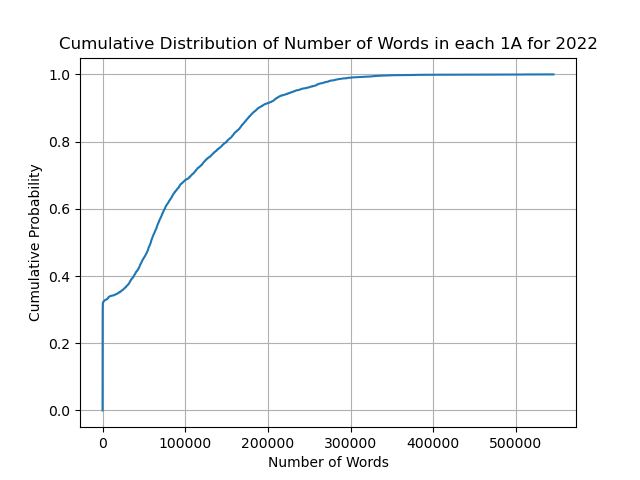
\includegraphics[width=\textwidth]{cdf_words}
	\caption{Cumulative Distribution of Number of Words}	
    \label{fig:figure1}
  \end{subfigure}
  \hfill
  \begin{subfigure}{0.45\textwidth}
    \centering
    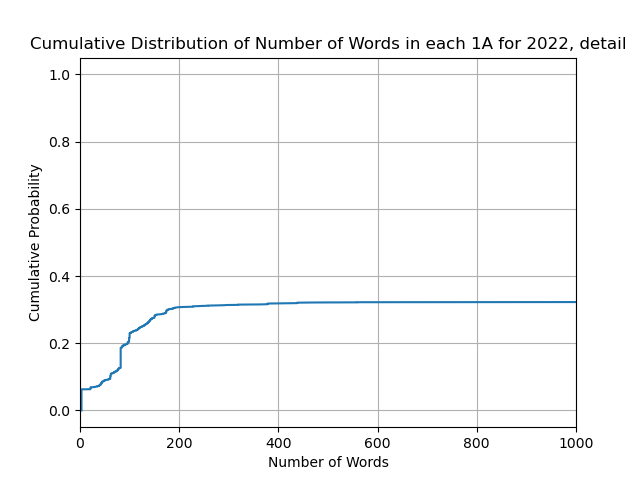
\includegraphics[width=\textwidth]{cdf_words_zoom}
	\caption{Cumulative Distribution of Number of Words, Zoom}
    \label{fig:figure2}
  \end{subfigure}
  \caption{Cumulative Distribution of Number of Words in 2022}
  \label{fig:cdf}
\end{figure}


\begin{table}[!htbp] \centering 

  \label{tab:file_counts} 
\begin{tabular}{@{\extracolsep{5pt}} D{.}{.}{-3} D{.}{.}{-3} D{.}{.}{-3} } 
\\[-1.8ex]\hline 
\hline \\[-1.8ex] 
\multicolumn{1}{c}{Year} & \multicolumn{1}{c}{Total\_1As} & \multicolumn{1}{c}{Filtered} \\ 
\hline \\[-1.8ex] 
\multicolumn{1}{c}{2006} & \multicolumn{1}{c}{5685} & \multicolumn{1}{c}{2466} \\ 
\multicolumn{1}{c}{2007} & \multicolumn{1}{c}{6445} & \multicolumn{1}{c}{2714} \\ 
\multicolumn{1}{c}{2008} & \multicolumn{1}{c}{6931} & \multicolumn{1}{c}{2305} \\ 
\multicolumn{1}{c}{2009} & \multicolumn{1}{c}{8244} & \multicolumn{1}{c}{2190} \\ 
\multicolumn{1}{c}{2010} & \multicolumn{1}{c}{8122} & \multicolumn{1}{c}{2290} \\ 
\multicolumn{1}{c}{2011} & \multicolumn{1}{c}{8019} & \multicolumn{1}{c}{2356} \\ 
\multicolumn{1}{c}{2012} & \multicolumn{1}{c}{7797} & \multicolumn{1}{c}{2316} \\ 
\multicolumn{1}{c}{2013} & \multicolumn{1}{c}{7560} & \multicolumn{1}{c}{2401} \\ 
\multicolumn{1}{c}{2014} & \multicolumn{1}{c}{7560} & \multicolumn{1}{c}{2518} \\ 
\multicolumn{1}{c}{2015} & \multicolumn{1}{c}{7531} & \multicolumn{1}{c}{2528} \\ 
\multicolumn{1}{c}{2016} & \multicolumn{1}{c}{7196} & \multicolumn{1}{c}{2431} \\ 
\multicolumn{1}{c}{2017} & \multicolumn{1}{c}{6896} & \multicolumn{1}{c}{2394} \\ 
\multicolumn{1}{c}{2018} & \multicolumn{1}{c}{6804} & \multicolumn{1}{c}{2418} \\ 
\multicolumn{1}{c}{2019} & \multicolumn{1}{c}{6683} & \multicolumn{1}{c}{2404} \\ 
\multicolumn{1}{c}{2020} & \multicolumn{1}{c}{6531} & \multicolumn{1}{c}{2332} \\ 
\multicolumn{1}{c}{2021} & \multicolumn{1}{c}{6936} & \multicolumn{1}{c}{2308} \\ 
\multicolumn{1}{c}{2022} & \multicolumn{1}{c}{6899} & \multicolumn{1}{c}{1885} \\ 
\hline \\[-1.8ex] 
\end{tabular} 
\caption{The left column shows the count of all 10-Ks retrieved for a given year. The right column counts all the 10-Ks that obey to the following filtering criteria: 1) Ordinary common shares; 2) Membership to NYSE, AMEX, and NASDAQ; 3) Price above \$ 5 in 2006 dollars; 4) Meaningful 10-K contents ($>$ 200 words)} 
\end{table} 
 

\subsection{Text conversion to bag-of-words}


After filtering firms, I utilize the \texttt{spacy} Python library to perform lemmatization on all filtered texts. Lemmatization is a technique used to convert words to their root form, thus ensuring semantic consistency. For example, variations like "take", "took", and "taken" are simplified to "take". \texttt{spacy} leverages WordNet, an extensive lexical database of English maintained by Princeton University.

In order to discern common collocations—like "patent application"—which impart more semantic depth compared to individual words, this study utilizes collocation detection as detailed in \cite{Mikolov2013-be}. This approach generates meaningful bigrams and trigrams. A minimum count threshold of 5 is established for collocations, ensuring that only statistically significant combinations are included in the dictionary.

The complete subset of words, bigrams, and trigrams found is used to create a dictionary, which 
 
Finally, I converted all texts to a bag-of-words format using the dictionary and the n-gramized texts. This format retains the count of appearances for each word in a document, $c_{ij}$, but disregards word order, resulting in the final representation of the corpus.

To further augment my analysis, I match firms based on their Central Index Key (CIK) and Permanent Company Number (PERMNO), linking their annual reports to several other data sources. This includes daily stock data (which I aggregate on a weekly basis), Compustat data, and measurements of the firms' knowledge capital, their accumulated patent value, and the level of skill in their respective industries as indicated by existing literature.

%Through this approach, I have observed a positive correlation between higher intensities of a specific topic, hereafter referred to as "topic\_kk", and the aforementioned measures. This suggests that firms that more frequently discuss this topic may have higher levels of knowledge capital, accumulated patent value, and industry skill.
%
%Furthermore, I have found that firms in the upper quartile of "topic\_kk" intensity have consistently outperformed their peers in terms of returns since 2006. This finding indicates a potential link between the subject matter discussed in firms' annual reports and their financial performance.



%TODO Create in R a function that receives one of the key df's 

%TODO Create in r a funciton that returns: for a given year; distr per topic; average K_int/K_int_Know per topic; average patent expenditure; average/std size  

% TODO: How many 1As per year? How many public firms in Compustat?

\subsection{Topic modeling}

Having the corpus and the dictionary, I apply unsupervised topic modeling, specifically using the Latent Dirichlet Allocation technique, to the entire corpus of documents. These documents contain risk factors for different firms over various years. As part of the model's setup, I set a parameter for the number of topics, denoted as \textit{k}, and feed the model with the dictionary I previously constructed. The choice of \textit{k} is often done \textit{ad hoc} and is primarily driven by interpretability, as noted by Gentzkow (2019).

An example of output from such a model is shown in Figure \ref{fig:bubble_plot}.

\insertfigure{bubble_plot}{A graphic representation of a four-topic model on firms' risk factors since 2006.}

After merging a four-topic map between firms and topic intensities to firms' identifying data, I obtain a topic map as shown in Table \ref{tab:topic_map}.

\begin{table}[!htbp] \centering 
  \caption{Sample of topic map} 
  \label{tab:topic_map} 
\begin{tabular}{@{\extracolsep{5pt}} D{.}{.}{-3} D{.}{.}{-3} D{.}{.}{-3} D{.}{.}{-3} D{.}{.}{-3} D{.}{.}{-3} D{.}{.}{-3} } 
\\[-1.8ex]\hline 
\hline \\[-1.8ex] 
\multicolumn{1}{c}{conm} & \multicolumn{1}{c}{year} & \multicolumn{1}{c}{CIK} & \multicolumn{1}{c}{topic\_0} & \multicolumn{1}{c}{topic\_1} & \multicolumn{1}{c}{topic\_2} & \multicolumn{1}{c}{topic\_3} \\ 
\hline \\[-1.8ex] 
\multicolumn{1}{c}{BOEING CO} & \multicolumn{1}{c}{2015} & \multicolumn{1}{c}{12927} & \multicolumn{1}{c}{0.875} & \multicolumn{1}{c}{0.109} & \multicolumn{1}{c}{0.016} & \multicolumn{1}{c}{0} \\ 
\multicolumn{1}{c}{UNIFI INC} & \multicolumn{1}{c}{2022} & \multicolumn{1}{c}{100726} & \multicolumn{1}{c}{0.893} & \multicolumn{1}{c}{0.107} & \multicolumn{1}{c}{0} & \multicolumn{1}{c}{0} \\ 
\multicolumn{1}{c}{UTAH MEDICAL PRODUCTS INC} & \multicolumn{1}{c}{2007} & \multicolumn{1}{c}{706698} & \multicolumn{1}{c}{0.021} & \multicolumn{1}{c}{0.457} & \multicolumn{1}{c}{0} & \multicolumn{1}{c}{0.519} \\ 
\multicolumn{1}{c}{SPOK HOLDINGS INC} & \multicolumn{1}{c}{2010} & \multicolumn{1}{c}{1289945} & \multicolumn{1}{c}{0.356} & \multicolumn{1}{c}{0.643} & \multicolumn{1}{c}{0} & \multicolumn{1}{c}{0} \\ 
\multicolumn{1}{c}{APTARGROUP INC} & \multicolumn{1}{c}{2015} & \multicolumn{1}{c}{896622} & \multicolumn{1}{c}{0.791} & \multicolumn{1}{c}{0.146} & \multicolumn{1}{c}{0} & \multicolumn{1}{c}{0.062} \\ 
\multicolumn{1}{c}{OASIS PETROLEUM INC} & \multicolumn{1}{c}{2018} & \multicolumn{1}{c}{1486159} & \multicolumn{1}{c}{1} & \multicolumn{1}{c}{0} & \multicolumn{1}{c}{0} & \multicolumn{1}{c}{0} \\ 
\multicolumn{1}{c}{PROGRESSIVE CORP-OHIO} & \multicolumn{1}{c}{2011} & \multicolumn{1}{c}{80661} & \multicolumn{1}{c}{0.051} & \multicolumn{1}{c}{0.238} & \multicolumn{1}{c}{0.711} & \multicolumn{1}{c}{0} \\ 
\multicolumn{1}{c}{RENTRAK CORP} & \multicolumn{1}{c}{2009} & \multicolumn{1}{c}{800458} & \multicolumn{1}{c}{0.017} & \multicolumn{1}{c}{0.982} & \multicolumn{1}{c}{0} & \multicolumn{1}{c}{0} \\ 
\multicolumn{1}{c}{UNVL STAINLESS  ALLOY PRODS} & \multicolumn{1}{c}{2015} & \multicolumn{1}{c}{931584} & \multicolumn{1}{c}{0.957} & \multicolumn{1}{c}{0.042} & \multicolumn{1}{c}{0} & \multicolumn{1}{c}{0} \\ 
\multicolumn{1}{c}{QUALCOMM INC} & \multicolumn{1}{c}{2015} & \multicolumn{1}{c}{804328} & \multicolumn{1}{c}{0} & \multicolumn{1}{c}{0.998} & \multicolumn{1}{c}{0} & \multicolumn{1}{c}{0} \\ 
\hline \\[-1.8ex] 
\end{tabular} 
\end{table} 



%Factors HML, SMB, and $Mkt-RF$ are extracted from Kenneth French's website. Intangible capital data is extracted from \cite	{Peters2017-fl}. The Fama-French 12 industry classification is used for the industry \texttt{ind12} factor when applicable. The stock return data is at a monthly frequency. The daily log-returns are converted to monthly by summing them. Excess return is then computed by taking the difference between the monthly return and the risk-free rate. The SP500 return is obtained using a proxy stock with CUSIP 78462F10. The beta for each stock is calculated using the formula $\beta = \frac{Var(ER_i)}{Cov(ER_i, ER_m)}$, where NAs are discarded. All relevant data, including industry information, is included in the dataframe \texttt{df\_full}. The total number of 10-Ks retrieved for each year is shown in Table \ref{filecounts}.


% TODO: Find out: what min_count to use? Does this actually make a large differnece? 

% TODO Need to change: re-run processes with \n detection

% TODO Need to change: re-run processes starting in 2005

% TODO Need to change: use default instead of npmi; min_count = 5; threshold = 10

\section{Results}

For every topic map, I define "topic\_kk" as the topic that has the highest loading within high-tech sectors in the economy, defined as SIC codes 283, 357, 466, 367, 382, 384, 737 (\cite{Brown2009-zp}) 


\begin{table}[!htbp] \centering 
  \caption{Topic averages by hi-tech status} 
  \label{fig:bytech} 
\begin{tabular}{@{\extracolsep{5pt}} D{.}{.}{-3} D{.}{.}{-3} D{.}{.}{-3} D{.}{.}{-3} D{.}{.}{-3} } 
\\[-1.8ex]\hline 
\hline \\[-1.8ex] 
\multicolumn{1}{c}{hi\_tech} & \multicolumn{1}{c}{topic\_0} & \multicolumn{1}{c}{topic\_1} & \multicolumn{1}{c}{topic\_2} & \multicolumn{1}{c}{topic\_3} \\ 
\hline \\[-1.8ex] 
\multicolumn{1}{c}{0} & \multicolumn{1}{c}{0.018} & \multicolumn{1}{c}{0.459} & \multicolumn{1}{c}{0.267} & \multicolumn{1}{c}{0.253} \\ 
\multicolumn{1}{c}{1} & \multicolumn{1}{c}{0.308} & \multicolumn{1}{c}{0.584} & \multicolumn{1}{c}{0.02} & \multicolumn{1}{c}{0.086} \\ 
\hline \\[-1.8ex] 
\end{tabular} 
\end{table} 


\insertfigure{topickk_distr.png}{The histogram bars represent the frequency of topic\_kk values, while the red dashed lines indicate the quartile dividers. }
  

The mean topic intensity by year is shown in Figure \ref{fig:mean_tiy}. The figure illustrates the consistent upward trend in the mean intensity of knowledge-capital related language among a firm's risk factors, starting from 2009. 

%\begin{figure}[h!]
%	\centering
%  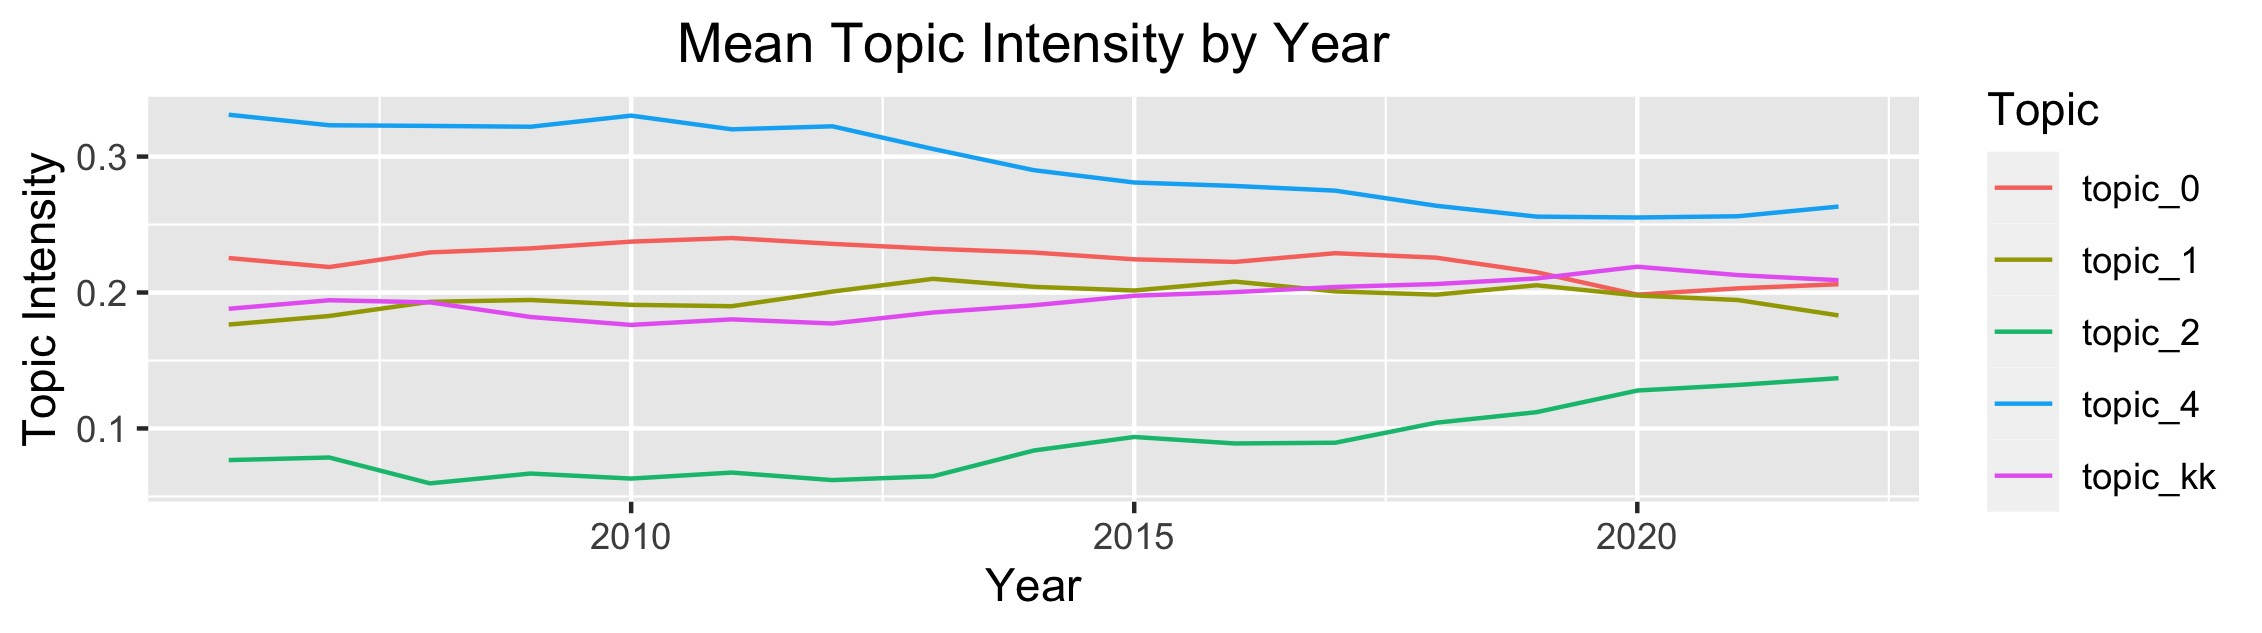
\includegraphics[width=0.8\textwidth]{\ffo/mean_tiy.jpg}
%  \caption{Mean topic intensity by year}
%  \label{fig:mean_tiy}
%\end{figure}
\insertfigure{mean_tiy}{Mean topic intensity by year}

I also analyze the performance of firms between differnet levels of knowledge-capital language. I create a varaible \texttt{kk\_bin}, which assumes values from 1 to 5, according to the topic's intensity (1 if between 0 and 0.2, 2 if between 0.2 and 0.4, up until 5, if between 0.8 and 1).

Figure \ref{fig:msdr} shows the monthly standard deviation of returns for the highest and lowest bins of the knowledge capital topic. Figure \ref{fig:awamr} shows the accumulated returns for each bin of the high knowledge capital topic.

% Table created by stargazer v.5.2.2 by Marek Hlavac, Harvard University. E-mail: hlavac at fas.harvard.edu
% Date and time: Thu, Jan 25, 2024 - 16:57:10
% Requires LaTeX packages: dcolumn 
\begin{table}[!htbp] \centering 
  \caption{Regression Summary} 
  \label{} 
\begin{tabular}{@{\extracolsep{5pt}}lD{.}{.}{-3} D{.}{.}{-3} } 
\\[-1.8ex]\hline 
\hline \\[-1.8ex] 
 & \multicolumn{2}{c}{\textit{Dependent variable:}} \\ 
\cline{2-3} 
\\[-1.8ex] & \multicolumn{2}{c}{Average returns} \\ 
\\[-1.8ex] & \multicolumn{1}{c}{(1)} & \multicolumn{1}{c}{(2)}\\ 
\hline \\[-1.8ex] 
 kkrhml & -0.001^{***} &  \\ 
  & (0.0004) &  \\ 
  & & \\ 
 HML & -0.003^{***} & -0.003^{***} \\ 
  & (0.0005) & (0.001) \\ 
  & & \\ 
 SMB & -0.0001 & 0.0001 \\ 
  & (0.0004) & (0.0004) \\ 
  & & \\ 
 Mkt.RF & 0.002 & 0.003^{*} \\ 
  & (0.002) & (0.002) \\ 
  & & \\ 
 Constant & 0.001 & -0.001 \\ 
  & (0.002) & (0.002) \\ 
  & & \\ 
\hline \\[-1.8ex] 
Observations & \multicolumn{1}{c}{36} & \multicolumn{1}{c}{36} \\ 
R$^{2}$ & \multicolumn{1}{c}{0.614} & \multicolumn{1}{c}{0.469} \\ 
Adjusted R$^{2}$ & \multicolumn{1}{c}{0.564} & \multicolumn{1}{c}{0.419} \\ 
Residual Std. Error & \multicolumn{1}{c}{0.00001 (df = 31)} & \multicolumn{1}{c}{0.00001 (df = 32)} \\ 
F Statistic & \multicolumn{1}{c}{12.322$^{***}$ (df = 4; 31)} & \multicolumn{1}{c}{9.405$^{***}$ (df = 3; 32)} \\ 
\hline 
\hline \\[-1.8ex] 
\textit{Note:}  & \multicolumn{2}{r}{$^{*}$p$<$0.1; $^{**}$p$<$0.05; $^{***}$p$<$0.01} \\ 
\end{tabular} 
\end{table} 
 

\insertfigure{awawr}{Asset-weighted accumulated weekly returns}

\insertfigure{wsdr_byg}{Weekly standard deviation of returns by group}

Table \ref{tab:bytech} shows the average topic intensity for low- and high-tech firms, as described by. 


\begin{table}[!htbp] \centering 
  \caption{Topic averages by hi-tech status} 
  \label{fig:bytech} 
\begin{tabular}{@{\extracolsep{5pt}} D{.}{.}{-3} D{.}{.}{-3} D{.}{.}{-3} D{.}{.}{-3} D{.}{.}{-3} } 
\\[-1.8ex]\hline 
\hline \\[-1.8ex] 
\multicolumn{1}{c}{hi\_tech} & \multicolumn{1}{c}{topic\_0} & \multicolumn{1}{c}{topic\_1} & \multicolumn{1}{c}{topic\_2} & \multicolumn{1}{c}{topic\_3} \\ 
\hline \\[-1.8ex] 
\multicolumn{1}{c}{0} & \multicolumn{1}{c}{0.018} & \multicolumn{1}{c}{0.459} & \multicolumn{1}{c}{0.267} & \multicolumn{1}{c}{0.253} \\ 
\multicolumn{1}{c}{1} & \multicolumn{1}{c}{0.308} & \multicolumn{1}{c}{0.584} & \multicolumn{1}{c}{0.02} & \multicolumn{1}{c}{0.086} \\ 
\hline \\[-1.8ex] 
\end{tabular} 
\end{table} 
 

Figure  \ref{fig:heatmap} creates the correlation between the intensity of each of the topics and the industry's  \cite{Belo2017-qi} average labor-skill level of employees in a given narrowly-defined industry. Figure \ref{fig:heatmap_patents} creates the correlation matrix between topic intensities and a firms' patent intensities, defined as the ratio between the firms' cumulated value of their patents as defined by \cite{Kogan2019-mw} and their total assets.

\insertfigure{heatmap}{Correlation matrix between topics and skill}

%\begin{figure}[h!]
%	\centering
%  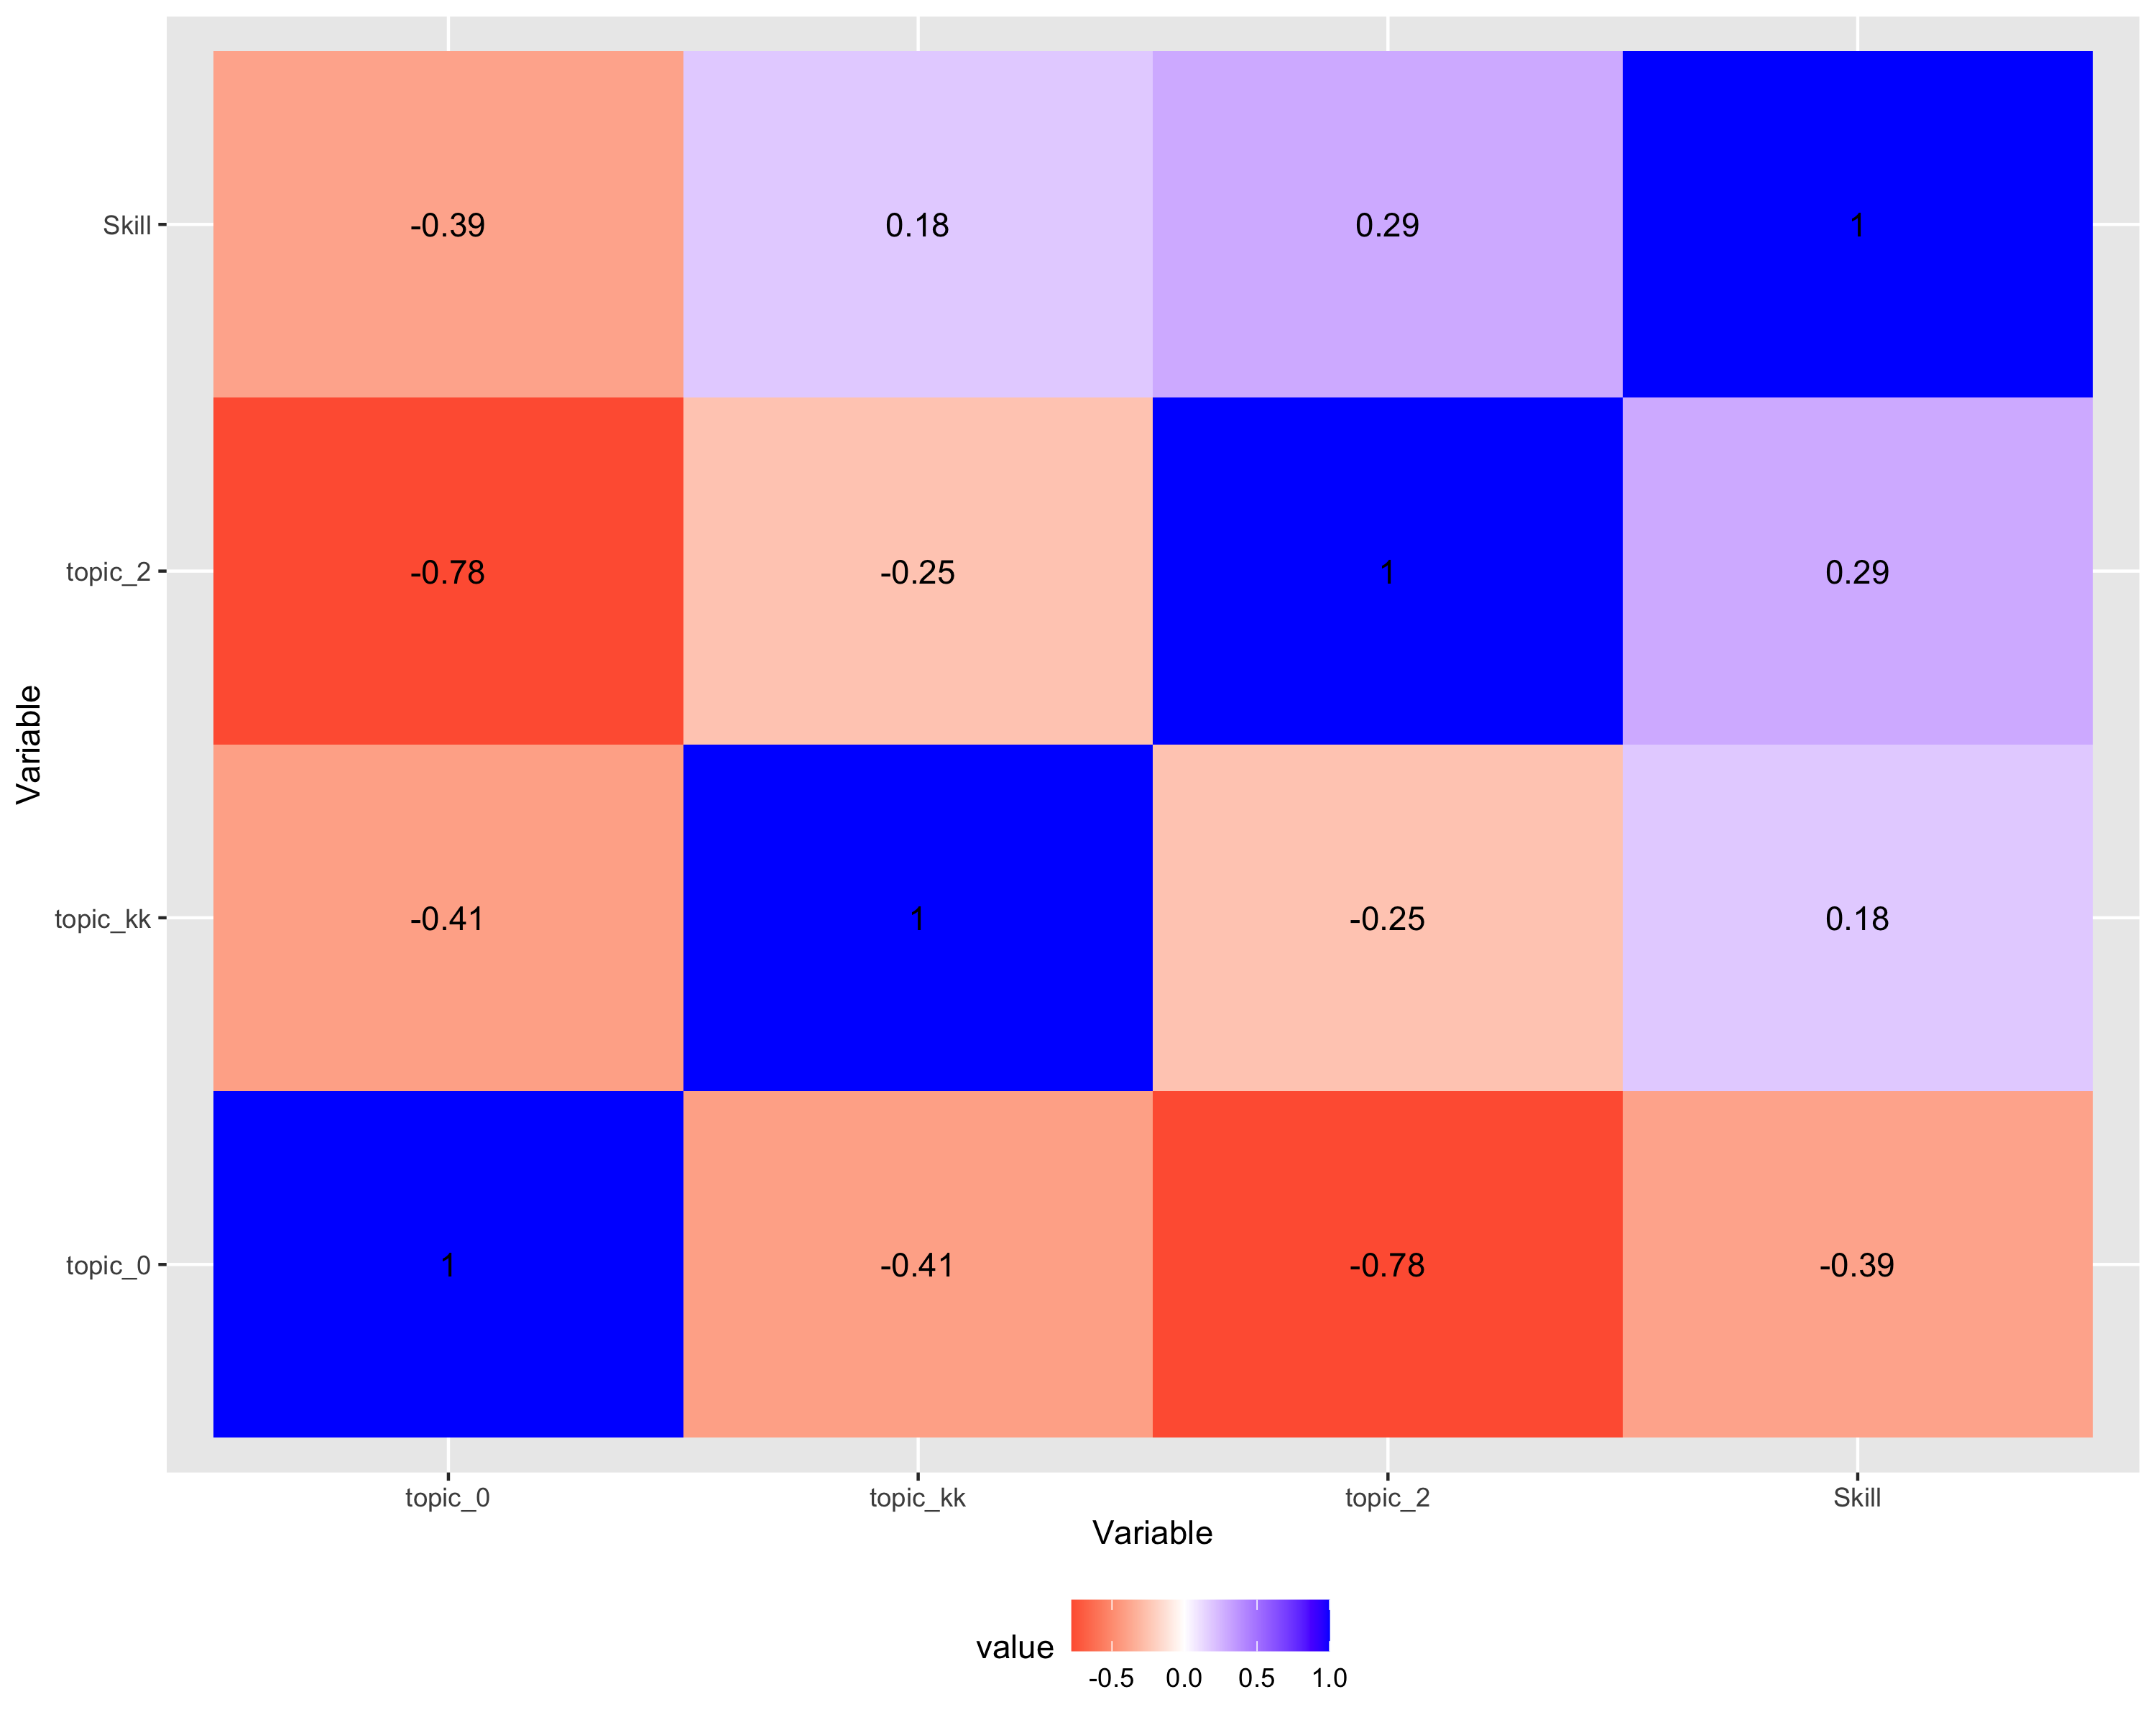
\includegraphics[width=0.8\textwidth]{\ffo/heatmap.png}
%  \caption{Correlation matrix between topics and skill}
%  \label{fig:heatmap}
%\end{figure}


\insertfigure{heatmap_patents}{Correlation matrix between topics and patent intensity}

%\begin{figure}[h!]
%	\centering
%  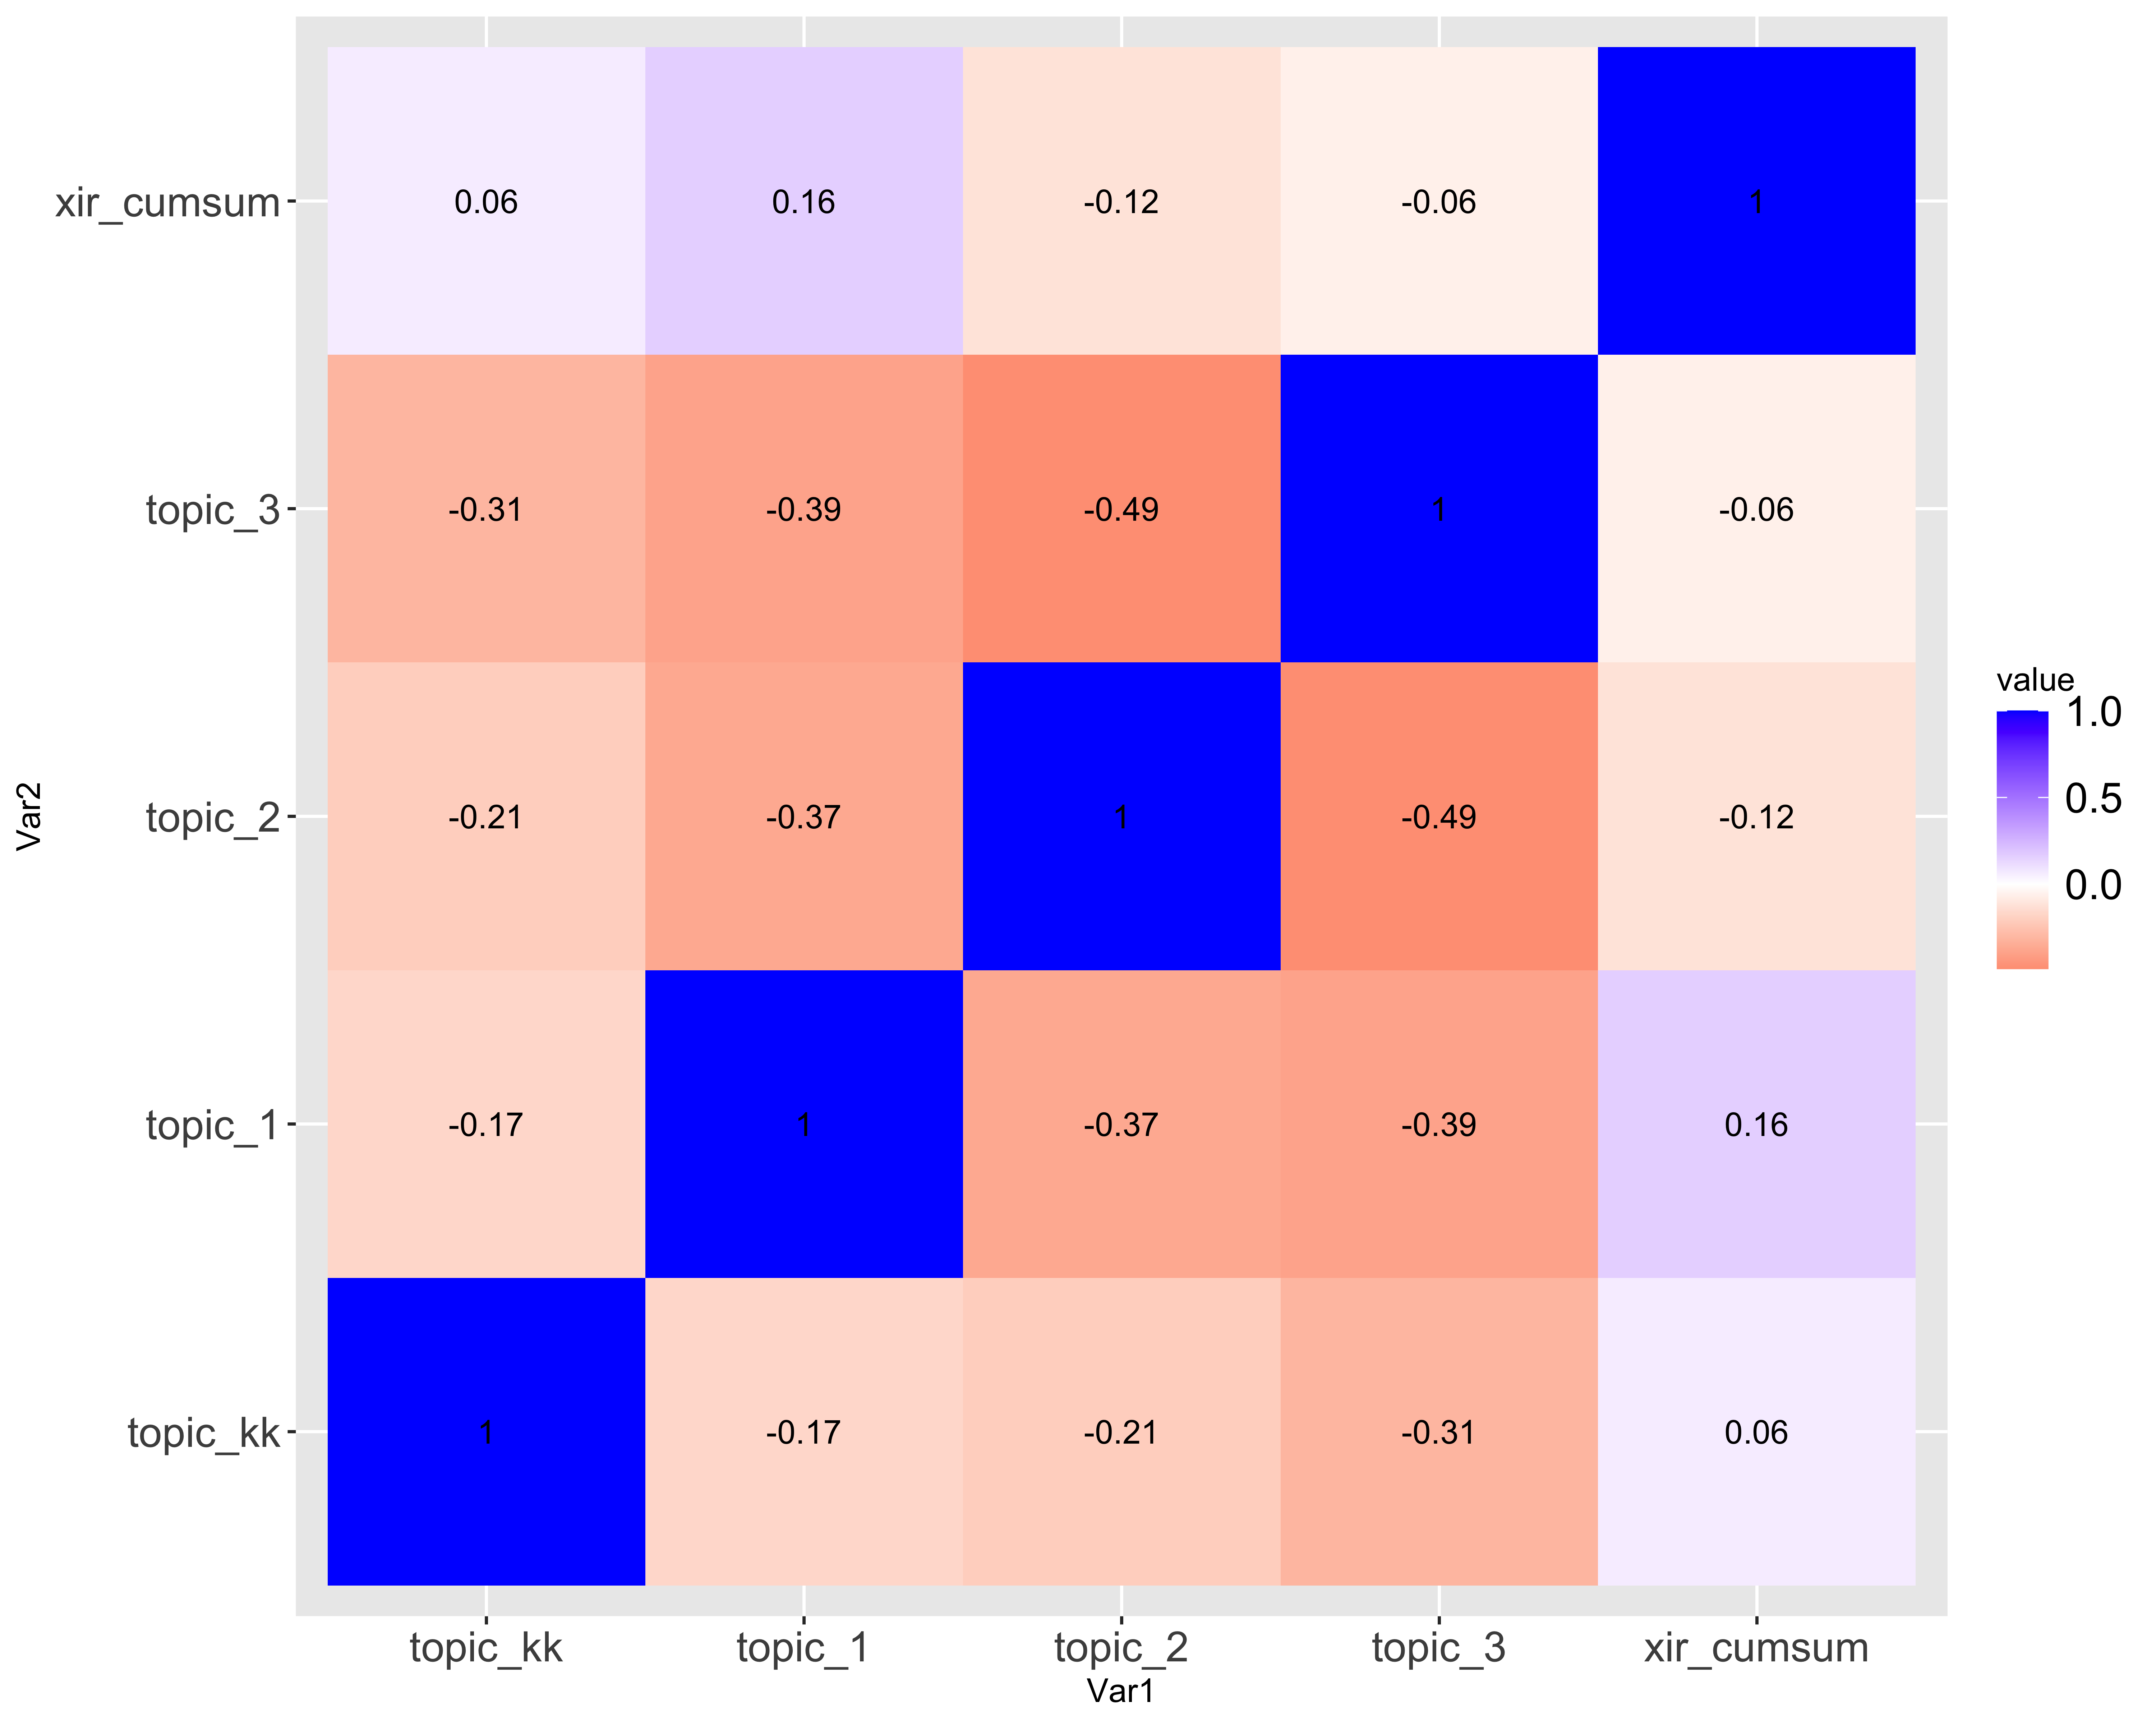
\includegraphics[width=0.8\textwidth]{\ffo/heatmap_patents.png}
%  \caption{Correlation matrix between topics and patent intensity}
%  \label{fig:heatmap_patents}
%\end{figure}



% Table created by stargazer v.5.2.2 by Marek Hlavac, Harvard University. E-mail: hlavac at fas.harvard.edu
% Date and time: Thu, Jan 25, 2024 - 16:57:10
% Requires LaTeX packages: dcolumn 
\begin{table}[!htbp] \centering 
  \caption{Regression Summary} 
  \label{} 
\begin{tabular}{@{\extracolsep{5pt}}lD{.}{.}{-3} D{.}{.}{-3} } 
\\[-1.8ex]\hline 
\hline \\[-1.8ex] 
 & \multicolumn{2}{c}{\textit{Dependent variable:}} \\ 
\cline{2-3} 
\\[-1.8ex] & \multicolumn{2}{c}{Average returns} \\ 
\\[-1.8ex] & \multicolumn{1}{c}{(1)} & \multicolumn{1}{c}{(2)}\\ 
\hline \\[-1.8ex] 
 kkrhml & -0.001^{***} &  \\ 
  & (0.0004) &  \\ 
  & & \\ 
 HML & -0.003^{***} & -0.003^{***} \\ 
  & (0.0005) & (0.001) \\ 
  & & \\ 
 SMB & -0.0001 & 0.0001 \\ 
  & (0.0004) & (0.0004) \\ 
  & & \\ 
 Mkt.RF & 0.002 & 0.003^{*} \\ 
  & (0.002) & (0.002) \\ 
  & & \\ 
 Constant & 0.001 & -0.001 \\ 
  & (0.002) & (0.002) \\ 
  & & \\ 
\hline \\[-1.8ex] 
Observations & \multicolumn{1}{c}{36} & \multicolumn{1}{c}{36} \\ 
R$^{2}$ & \multicolumn{1}{c}{0.614} & \multicolumn{1}{c}{0.469} \\ 
Adjusted R$^{2}$ & \multicolumn{1}{c}{0.564} & \multicolumn{1}{c}{0.419} \\ 
Residual Std. Error & \multicolumn{1}{c}{0.00001 (df = 31)} & \multicolumn{1}{c}{0.00001 (df = 32)} \\ 
F Statistic & \multicolumn{1}{c}{12.322$^{***}$ (df = 4; 31)} & \multicolumn{1}{c}{9.405$^{***}$ (df = 3; 32)} \\ 
\hline 
\hline \\[-1.8ex] 
\textit{Note:}  & \multicolumn{2}{r}{$^{*}$p$<$0.1; $^{**}$p$<$0.05; $^{***}$p$<$0.01} \\ 
\end{tabular} 
\end{table} 
 
\FloatBarrier
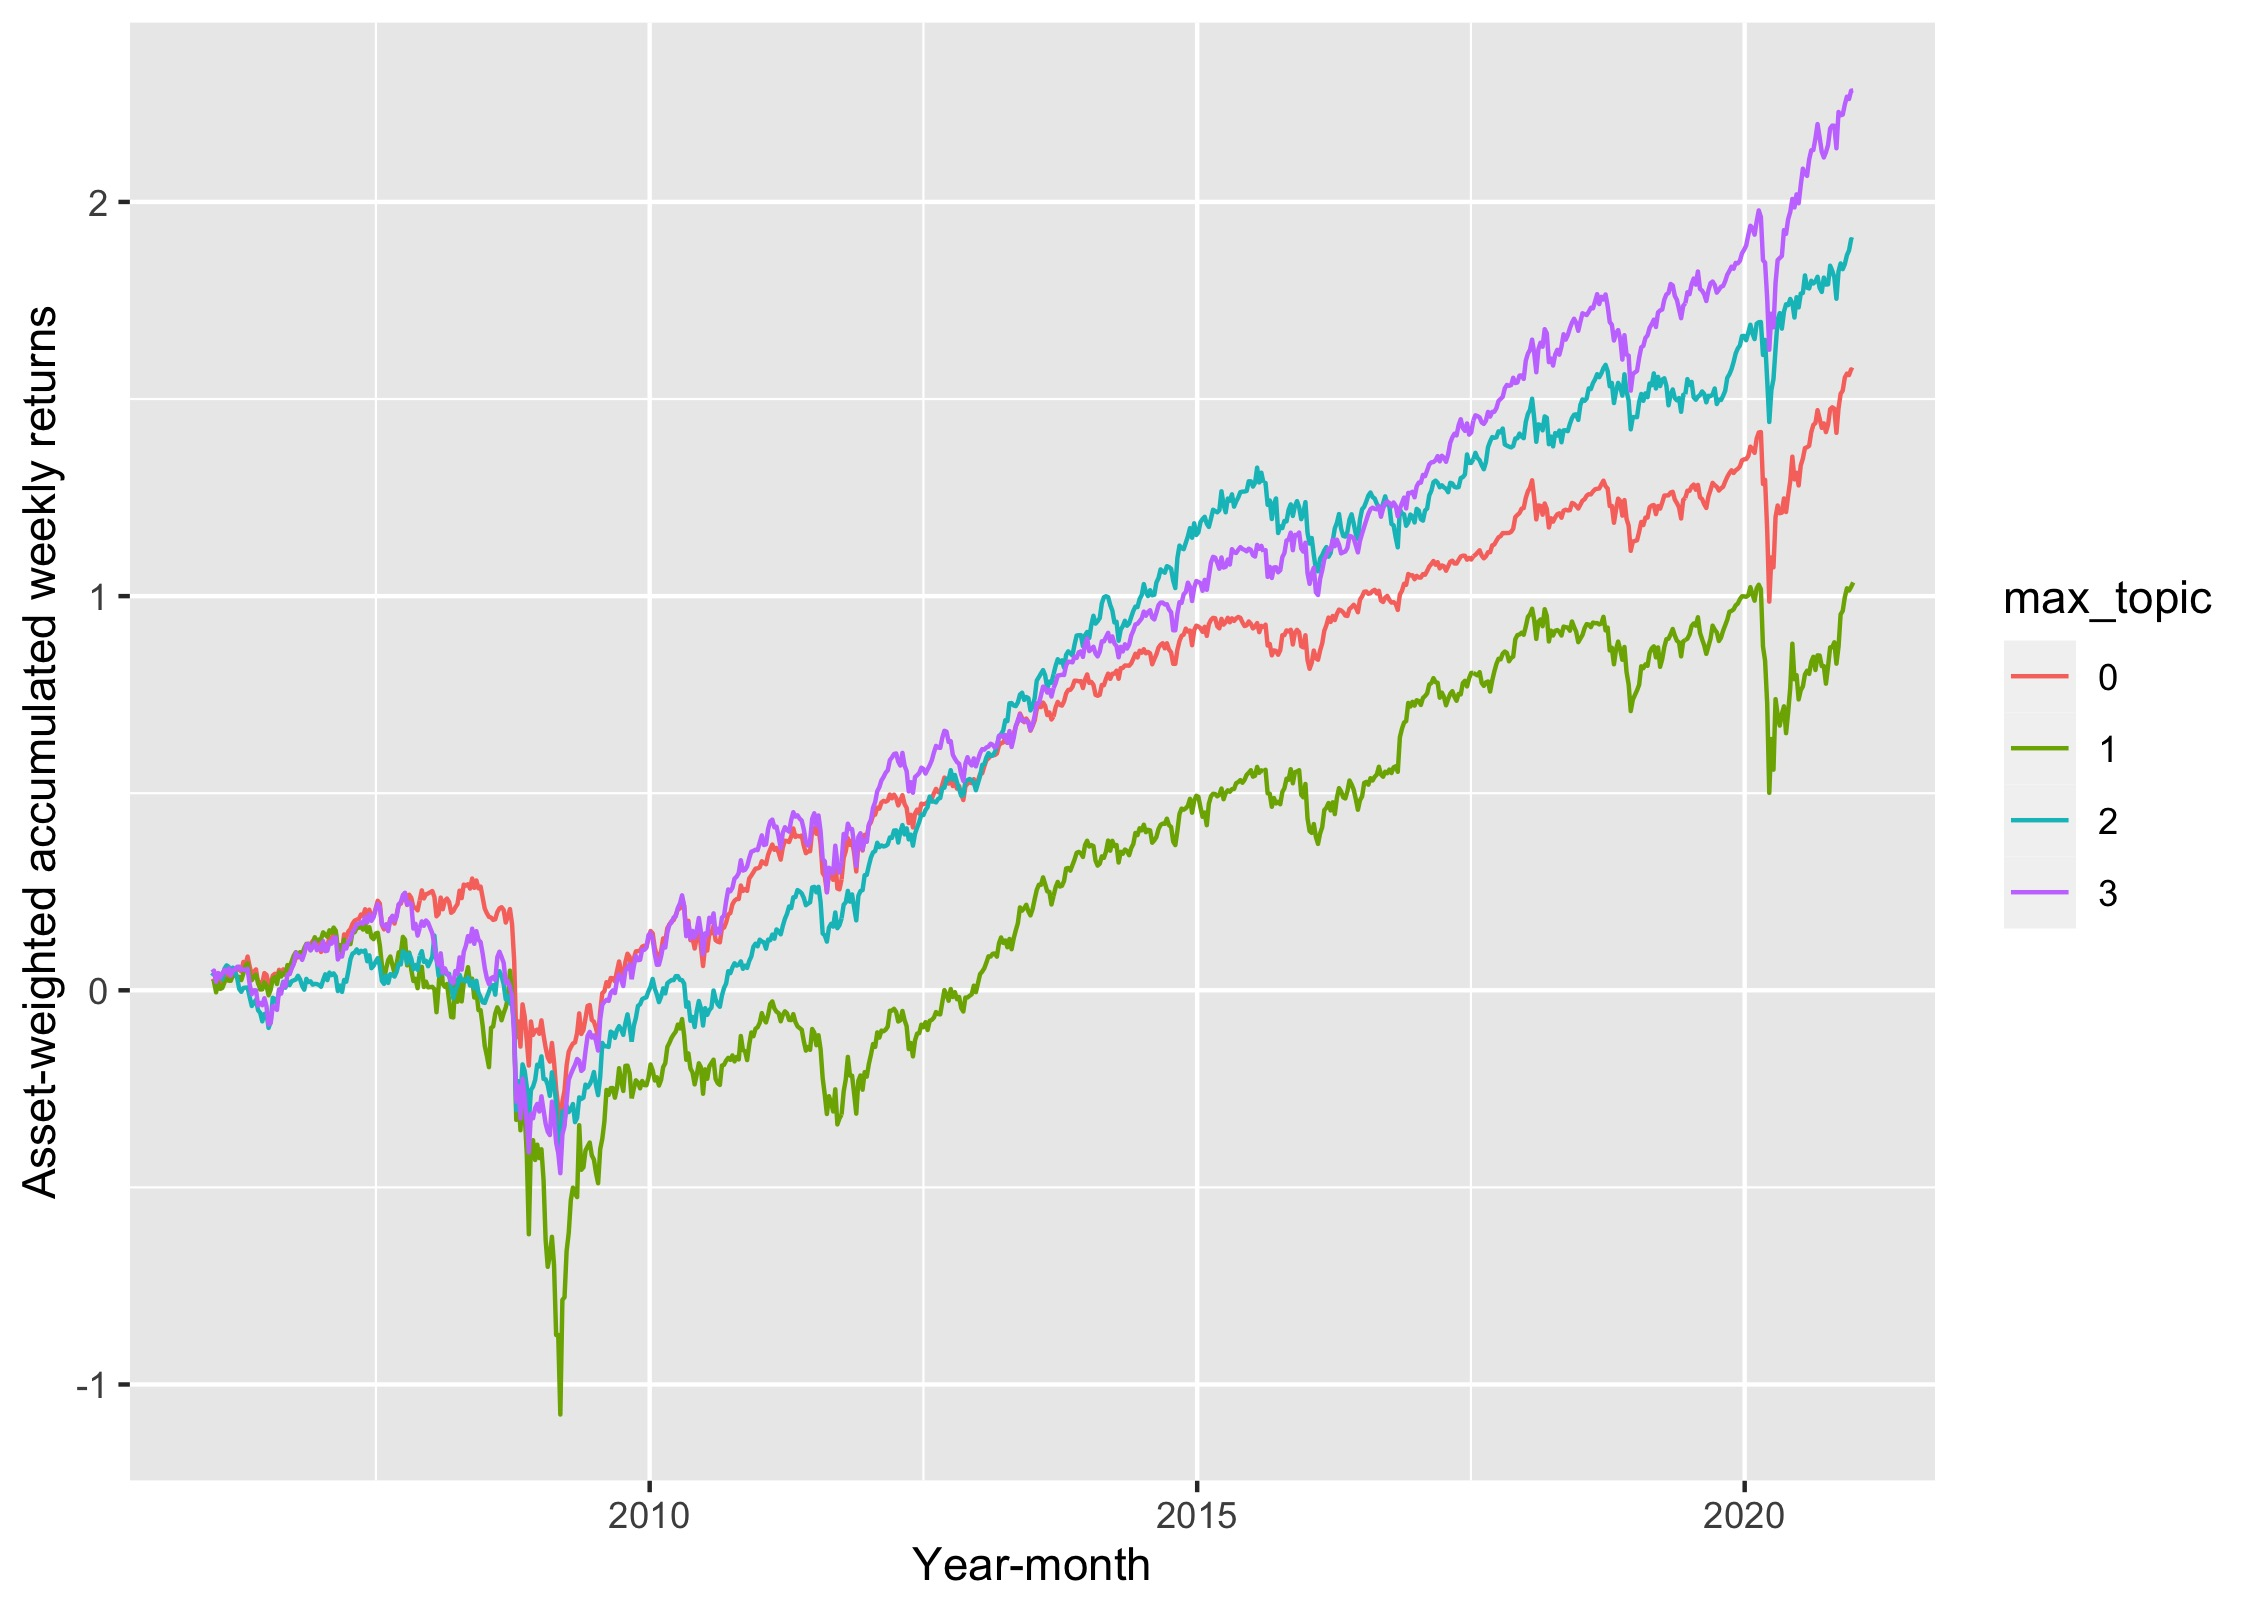
\includegraphics[width=0.6\textwidth]{\ffo/awawr_byg.jpg}
\FloatBarrier

\insertfigure{stackedplot_at}{Stacked plot of firms' total assets in the upper quartile of KK topic intensity}

\insertfigure{stackedplot_n}{-}

\insertfigure{topicvsikpt_hm}{-}

\insertfigure{topicvskkpt_hm}{-}


%
%The following calculations and categorizations are made:
%
%\begin{itemize}
%\item Market-to-book ratios (\texttt{mb}) are found using the formula: \texttt{mb = (csho * prcc\_f) / ceq}, where \texttt{csho} represents common shares outstanding, \texttt{prcc\_f} represents the closing price of the stock, and \texttt{ceq} represents common equity.
%\item Market equity is calculated as the product of \texttt{csho} and \texttt{prcc\_f}.
%\item Stocks are divided into \texttt{r ndim\_mb} groups based on their market-to-book ratio.
%\item Stocks are also divided into \texttt{r ndim\_me} groups based on their market equity.
%\item Stocks are categorized into \texttt{r ndim\_kkc} groups based on their membership in the knowledge-capital-heavy cluster.
%\item Returns for each portfolio, which are divided into two dimensions, are calculated as the asset-weighted sum of returns using \texttt{ff3\_ret}.
%\item Returns for each portfolio, which are divided into three dimensions, are calculated as the asset-weighted sum of returns using \texttt{ff3\_wKKc\_ret}.
%\item SMB (Small Minus Big) is the difference between the simple average of the returns on the three small stock portfolios and the average of the three big stock portfolios.
%\item HML (High Minus Low) is the difference between the simple average of the returns on the two low market-to-book (MB) portfolios (high book-to-market ratio) and the two high MB portfolios (low book-to-market ratio).
%\end{itemize}
%
%Considering knowledge capital risk a non-traded factor, I run the regression in two stages. In the first one, I obtain estimates of betas from the time-series regression:
%
%\begin{equation}
%\bar{ER}_t = a + \beta_{SMB, t} SMB_t + \beta_{HML, t} HML_t + \beta_{KKHML, t} KKHML_T + \beta_{ERM, t} (RM_t - RF_t) +\varepsilon_t
%\end{equation}
%
%In the second stage, I obtain a cross-sectional regression of average returns on betas. The betas here are the explanatory variables. Since the regression residuals are cross-sectionally correlated, I also run WLS, using as weights the variance of residuals for each portfolio.
%
%Stocks were grouped monthly into 12 portfolios based on three dimensions: book-to-market ratio (L, M, H), market value (S, B), and knowledge risk intensity (H, L). Book-to-market was divided into terciles (L, M, H), while market value was divided using the median (S, B). High knowledge risk intensity was determined based on cluster 1 in an LDA analysis, with other firms categorized as 0.
%
%$$
%R_{i,t} - R_{f,t} = \beta_{1,i} HML_{t} + \beta_{2,i} SMB_{t} + \beta_{3,i} KKHML_{t} + \epsilon_{i,t}
%$$
%
%Each of the tables below include coefficients for 12 stock portfolios formed on size (S/B), book-to-market equity (H/M/L), and KK loading (H/L).
%
%The graph below illustrates the monthly returns of high- and low-knowledge firms, presented as the mean asset-weighted returns. Additionally, the subsequent graph displays the standard deviation of monthly returns for the respective groups, providing further insight into their performance. It is clear that high-knowledge firms have been more volatile throughout the times, with the notable exception of March 2020.


\bibliography{mylibrary2}

\end{document} 